\begin{activity} \label{A:11.3.2} Consider the iterated integral $\ds \int_{x=3}^{x=5} \int_{y=-x}^{y=x^2} (4x+10y) \, dy \, dx$.
    \ba
    \item Sketch the region of integration, $D$, for which 
    $$\ds \iint_D (4x + 10y) \, dA = \int_{x=3}^{x=5} \int_{y=-x}^{y=x^2} (4x+10y) \, dy \, dx.$$

    \item Determine the equivalent iterated integral that results from integrating in the opposite order ($dx \, dy$, instead of $dy \, dx$).  That is, determine the limits of integration for which 
$$\ds \iint_D (4x + 10y) \, dA = \int_{y=?}^{y=?}  \int_{x=?}^{x=?} (4x+10y) \, dx \, dy.$$
    \item Evaluate one of the two iterated integrals above. Explain what the value you obtained tells you.
    
    \item Set up and evaluate a single definite integral to determine the exact area of $D$, $A(D)$.
    
    \item Determine the exact average value of $f(x,y) = 4x  + 10y$ over $D$.

    \ea

\end{activity}
\begin{smallhint}

\end{smallhint}
\begin{bighint}

\end{bighint}
\begin{activitySolution}
   \ba
    \item The region $D$ of integration has $-x \leq y \leq x^2$ and $3 \leq x \leq 5$. This region is as shown in the figure below.
\begin{center}
\resizebox{!}{2.0in}{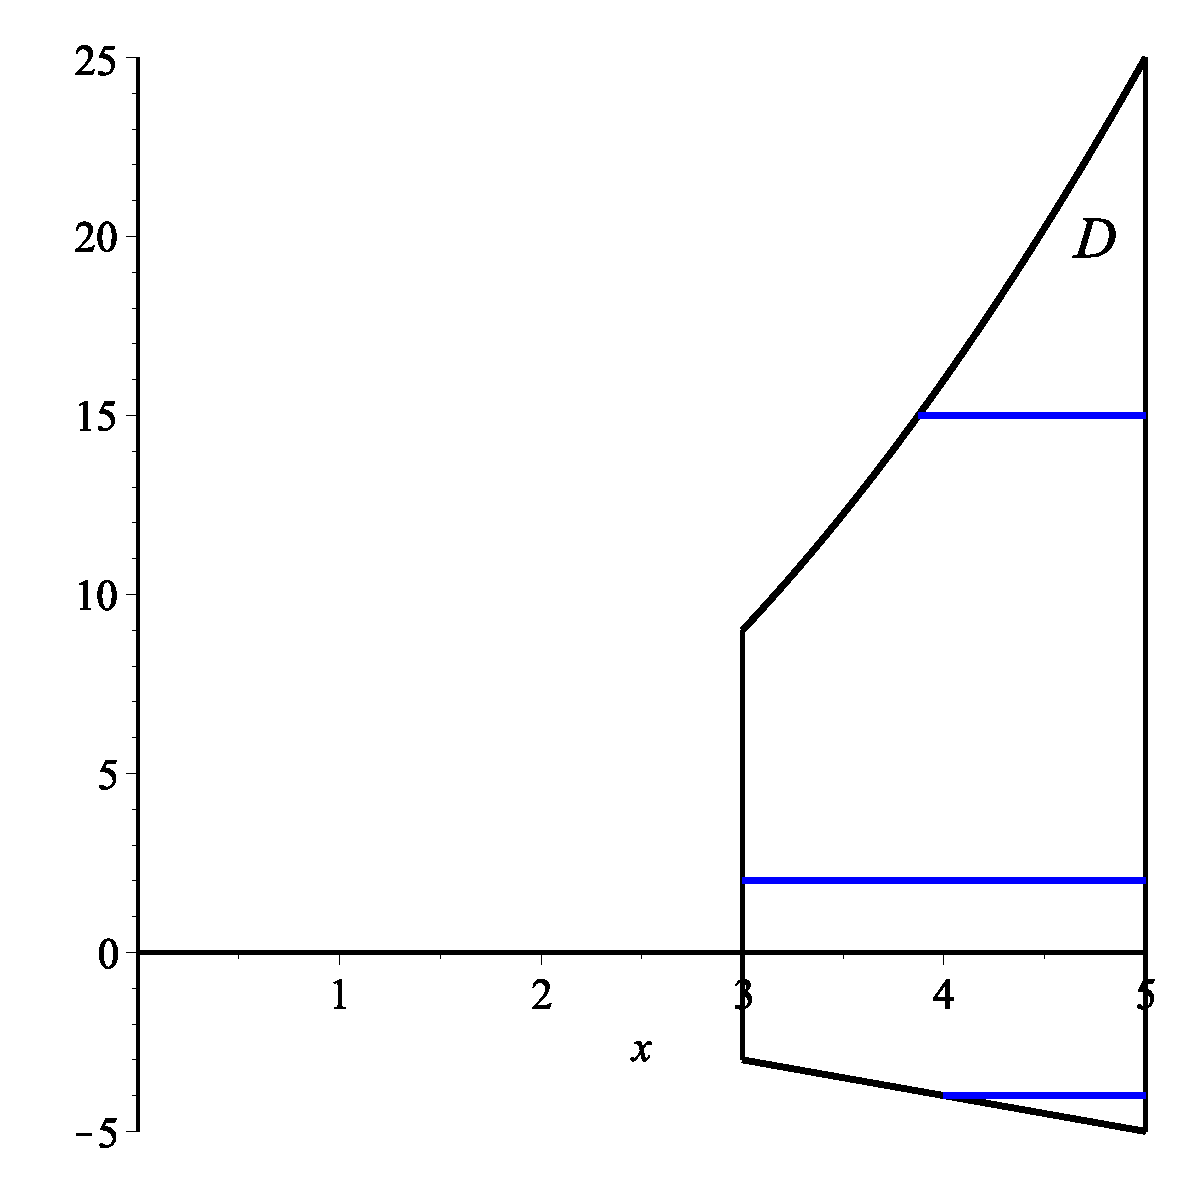
\includegraphics{11_3_Act_2}}
\end{center}


    \item If we integrate with respect to $x$ first, then $y$, the cross sections in the $x$-direction will always have their right endpoints on the line $x=5$. However, the left endpoints change as shown in the figure above. At the bottom of the figure, $x$ runs from $-y$ to $5$ for $y$ between $-3$ and $-5$. In the middle, $x$ runs between $x=3$ and $x=5$ for $y$ between $-3$ and $9$. At the top, $x$ runs from $\sqrt{y}$ to $x=5$ for $y$ between $9$ and $25$. So a sum of  iterated integrals that gives the same value as the given iterated integral is 
\[\int_{-5}^{-3} \int_{-y}^{5} (4x+10y) \, dx \, dy + \int_{-3}^{9} \int_{3}^{5} (4x+10y) \, dx \, dy + \int_{9}^{25} \int_{\sqrt{y}}^{5} (4x+10y) \, dx \, dy.\]

    \item Evaluating the original integral yields
\begin{align*}
\int_3^5 \int_{-x}^{x^2} (4x+10y) \, dy \, dx &= \int_3^5 \left. \left[4xy+5y^2\right] \right|_{-x}^{x^2} \, dx \\
	&= \int_3^5  \left[\left(4x^3+5x^4\right) - \left(-4x^2+5x^2\right)\right] \, dx \\
	&= \int_3^5  \left[5x^4+4x^3-x^2\right] \, dx \\
	&= \left. \left[x^5+x^4-\frac{x^3}{3}\right] \right|_3^5  \\
	&= \frac{11125}{3} - 315 \\
	&= \frac{10180}{3}.
\end{align*}

Since $4x+10y \geq 0$ on this domain, the value obtained tells us the volume of the solid bounded above by the graph of the plane $4x+10y$ and below by the region of integration. 

\item The area of $D$ is found by integrating 1 over the domain $D$, or
\begin{align*}
A(D) &= \iint_D 1 \, dA \\
	&= \int_{x=3}^{x=5} \int_{y=-x}^{y=x^2} 1 \, dy \, dx \\
	&= \int_3^5  \left[x^2+x\right] \, dx \\
	&= \left. \left[\frac{x^3}{3}+\frac{x^2}{2}\right] \right|_3^5  \\
	&= \left[\frac{125}{3} + \frac{25}{2}\right] - \left[\frac{27}{3}+\frac{9}{2}\right] \\
	&= \frac{122}{3}.
\end{align*}

\item The average value of $f$ on $D$ is 
\[\frac{1}{A(D)} \iint_D f(x,y) \, dA = \frac{3}{122}\left(\frac{10180}{3}\right) = \frac{5090}{61}.\]

    \ea
\end{activitySolution}
\aftera
